\chapter{Service Instructions for the Mortising Head \\
SCHAUBLIN 13 \small(Accessory No. 1200)}


\section*{Main Features}

\begin{tabular}{@{}ll@{}}
    Adjustable stroke            & 0 to 60 mm      \\
    Number of strokes per minute & 60--430         \\
    Tilt                         & \(\pm90^\circ\) \\
    Chisel dimensions            & 12 x 12 mm      \\
\end{tabular}

\section*{Cleaning, Lubrication, and Maintenance}
Upon receipt and during use, the general instructions provided for the machine must be observed.
The mortising head includes 3 oilers for pressure lubrication using the pump supplied with the machine.

\section*{Installation}
The mortising head is centered and secured by the two support arms (7).
For installation, insert the gear rack (154) provided with the mortising head into the spindle nose, then tighten it using the tightening key.
Extend one of the support arms (7) by approximately 250 mm, lock the front screw (5), mount the mortising head on the freed arm, unlock the screw (5), and insert the second support arm into the corresponding bore of the mortising head.

This mounting procedure avoids jamming that may occur during the simultaneous engagement of both support arms.
Press the mortising head against the face of the spindle head, taking care not to damage the gear teeth.
Secure the support arms (7) using the two screws (5) and tighten the screw (80) by pressing the mortising head firmly against the spindle head to prevent any torsion.
Finally, lock the two fixing screws (81).

The number of strokes must be limited to 430, which corresponds to a spindle speed of 405 rpm.

\begin{figure}[h]
    \centering
    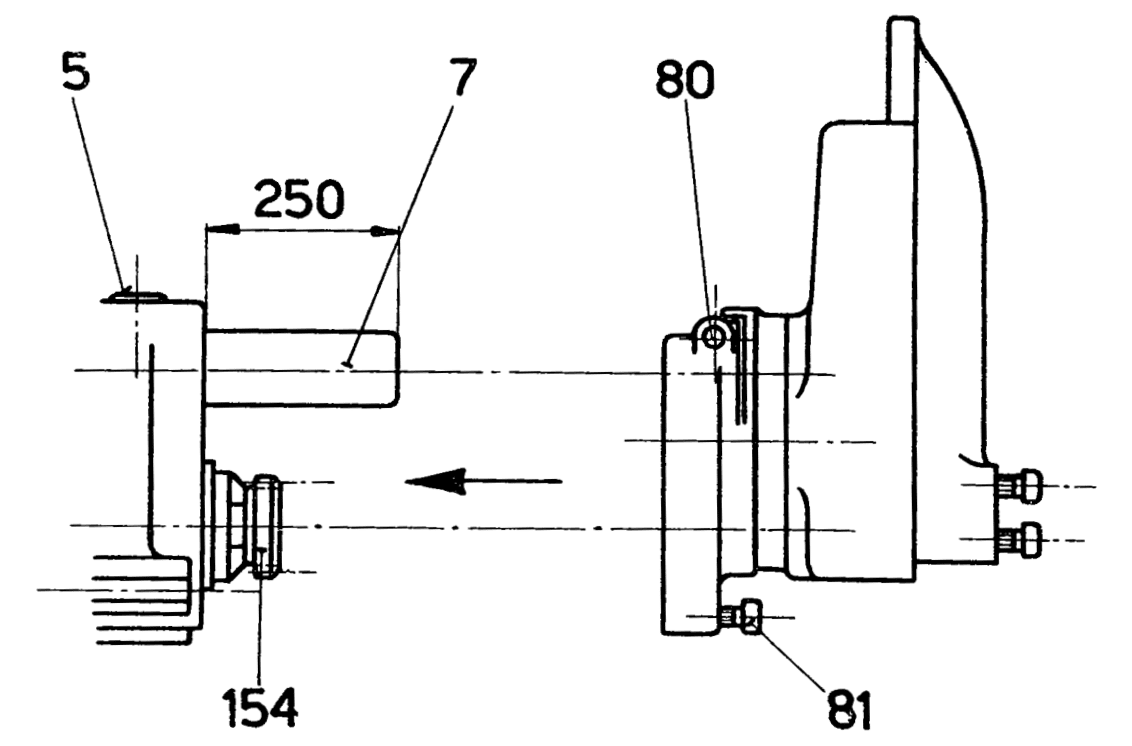
\includegraphics[width=0.7\linewidth]{images/page_37}
    \caption{Mortising Head Installation}
    \label{fig:mortising_head_installation}
\end{figure}
